\documentclass{article}
\usepackage{graphicx}
\usepackage{amsmath}
\usepackage{amsfonts}
\usepackage{algorithm}
\usepackage{algpseudocode}
\usepackage{caption}
\usepackage{subcaption}
\usepackage{import}
\usepackage{subcaption}
\usepackage{mathtools}
\usepackage[bookmarks]{hyperref}


\usepackage{fancyhdr}
\usepackage[a4paper, total={6in, 8in}]{geometry}

\graphicspath{./assets/}

\title{Performance Analysis of TSP Solving Techniques}
\author{Basaglia Alberto, Stocco Andrea}
\date{\today}

\begin{document}

\begin{titlepage}
    \centering
    \vspace*{\fill}

    \vspace*{0.5cm}

    \huge\bfseries
        Performance Analysis of TSP Solving Techniques

    \vspace*{0.5cm}

    \large Basaglia Alberto and Stocco Andrea

    \vspace*{2cm}

    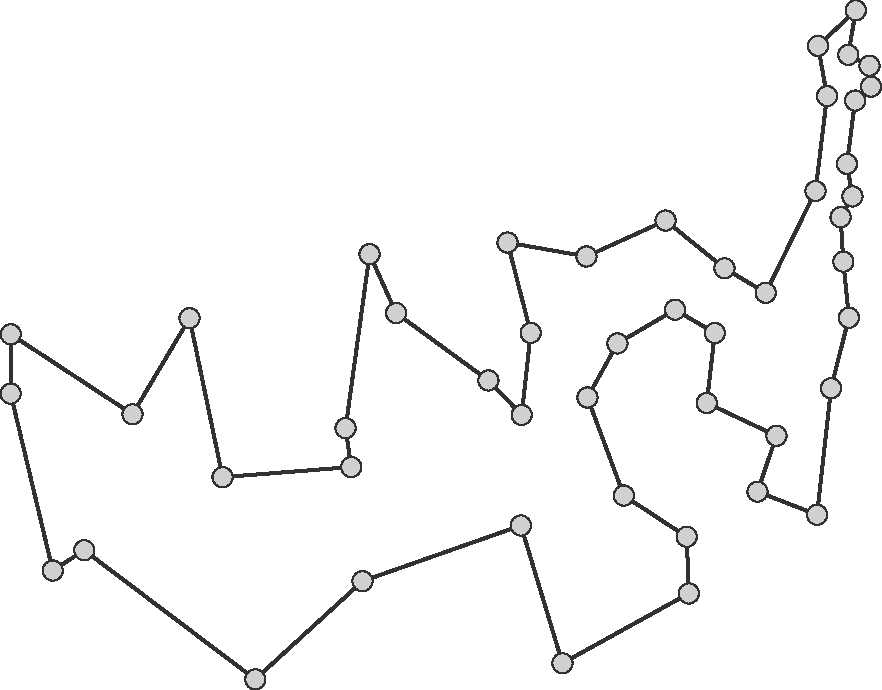
\includegraphics[width=12cm]{assets/cover.pdf} % also works with logo.pdf


    \vspace*{\fill}
\end{titlepage}

\newpage

\begin{abstract}
The Traveling Salesman Problem (TSP) is definitely one of the most intensively studied problems in optimization.
It asks the following question:
\textit{Given a list of cities and the distances between each pair of cities, what is the shortest possible route
that visits each city exactly once and returns to the origin city?}
TSP is computationally difficult (NP-Hard), but there exist many \textit{heuristics} and \textit{exact methods} to solve it.
In this report we are going to show and compare the performances of these
techniques.
\end{abstract}

\newpage
\tableofcontents
\newpage

\pagestyle{fancy}

\section{Introduction}
The Traveling Salesman Problem is for sure one of the most intensively studied problems in
optimization. The TSP asks the question of what is the shortest path that visits exactly
once all the nodes in a graph.
We can also define it as finding the shortest Hamiltonian path of a graph.

The problem was formulated mathematically by the Irish mathematician William Rowan
Hamilton and by the British mathematician Thomas Kirkman in the 19th century~\cite{biggs1986graph}.

The state of the art for solving the TSP problem nowadays is definitely the Concorde
software. Concorde was created by  D. Applegate, R.E. Bixby, V. Chvátal, and W.J. Cook.
It employs advanced combinatorial optimization techniques, linear programming, and cutting-plane methods~\cite{applegate1998solution}\cite{tuHu2022analyzing}.

The objective of this report is not to invent some new techniques that can compete with Concorde,
but instead to cover basic approaches, that can be implemented without much effort, and still lead
to good results.

\section{Heuristics}
Heuristics are algorithms to determine a near-optimal solution to an optimization problem. In certain scenarios,
exact methods aren't able to provide the optimal solution in a reasonable amount of time or they can't find it
at all. In contrast, a heuristic is generally capable of offering a solution that is more or less close to
the optimal one.
While there is no assurance regarding the optimality of the provided solution, it may still be considered
acceptable in some instances.

\subsection{Greedy}
A greedy algorithm is a heuristic that attempts to find an optimal solution by selecting the locally best possible choice at each iteration.
For instance, in our case, when determining the next node to visit, the greedy algorithm will always choose
the nearest unvisited one. Algorithm~\ref{alg:greedy} shows the pseudocode of this procedure

\begin{algorithm}[ht]
\caption{Greedy}
\label{alg:greedy}
\hspace*{0.5em} \textbf{Output}: $solution$
\begin{algorithmic}
\Procedure{greedy}{$startingnode, nnodes$}
	\State $solution \gets {0, 1, \dots, nnodes - 1}$
	\State $solution \gets \Call{swap}{solution, 0, startingnode}$
        \For{$i \gets 0$ to $nnodes - 1$}
                \State $mindist \gets \infty$
                \State $minindex \gets -1$
                \For{$j \gets i + 1$ to $nnodes$}
                        \If{$dist(i, j) < mindist$}
                                \State $mindist \gets dist(i, j)$
                                \State $minindex \gets j$
                        \EndIf
                \EndFor
                \State $solution \gets \Call{swap}{solution, i + 1, minindex}$
        \EndFor
\EndProcedure
\end{algorithmic}
\end{algorithm}
If we run this approach on an instance having the cities on a 2d plane and using the
eucledian distance as the cost of the edges, we will se, with a very high probability, an
high number of edges crossing.
It is possible to prove that an optimal solution, in this context, should not contain any crossing
between edges.
This fact can give us the intuition that a very simple yet clever technique could be used
to drastically improve our solution. This technique, known as \textit{2-opt}, will be covered
in the next section.

Another important point to discuss is the node the algorithm is started on.
One of the strategies we could think of would be to generate one randomly.
Although feasible, in our experiment we decided to run the greedy procedure
on all the possible starting nodes and then keep the best.


\subsection{2-opt}
The 2-opt algorithm is an optimization technique that can be used to improve a sub-optimal solution.
It evaluates the possibility of removing two edges in the tour and reconnecting the now disconnected nodes in the other way.
This process aims to improve the cost of the tour by eliminating inefficient segments while preserving the overall tour structure. By
iteratively exploring these adjustments and accepting them if they result in a shorter tour cost, the algorithm gradually refines
the solution. This iterative refinement continues until no further improvements can be made, resulting in a
solution closer to the optimal one for the given problem instance.
Although it is not the only possible situation where a 2-opt move is
beneficial, figure~\ref{fig:2optmove} illustrates an example of such a move.

\begin{figure}[H]
        \caption{Example of a 2-opt move}
        \label{fig:2optmove}
        \centering
        \begin{subfigure}{.5\textwidth}
                \centering
                \def\svgwidth{.7\linewidth}
                \import{assets}{2opt-pre.pdf_tex}
                \caption{Before the move}
        \end{subfigure}%
        \begin{subfigure}{.5\textwidth}
                \centering
                \def\svgwidth{.7\linewidth}
                \import{assets}{2opt-post.pdf_tex}
                \caption{After the move}
        \end{subfigure}
\end{figure}

It's easy to see that the removal of the crossing edges is beneficial to the
cost of the solution.

Algorithm \ref{alg:greedy_2opt} shows a possible implementation of this procedure to improve
the solution found with the greedy approach. In this case, as discussed in the
previous section, the greedy procedure is executed for every possible node.
Then, for each of the solutions, the \textit{2-opt} procedure is applied.
Another approach, that would use \textit{2-opt} only once instead of $n$ times, would be
to compute greedy on all the starting nodes first, and then \textit{2-opt} only on the
best one. This approach won't be covered in this report.

\begin{algorithm}[ht]
\caption{Best 2-opt Swap}
\label{alg:best2optswap}
\hspace*{0.5em} \textbf{Output}: $bestsolution$
\begin{algorithmic}
\Procedure{best2optswap}{$solution, nnodes$}
\State $bestsolution \gets solution$
        \For{$i \gets 0$ to $nnodes - 2$}
                \For{$j \gets i + 2$ to $nnodes$}
                        \State $newsolution \gets \Call{reversesubsequence}{solution, i + 1, j}$
                        \If{$\Call{cost}{newsolution} < \Call{cost}{bestsolution}$}
                                \State $bestsolution \gets newsolution$
                        \EndIf
                \EndFor
        \EndFor
\EndProcedure
\end{algorithmic}
\end{algorithm}

\begin{algorithm}[ht]
\caption{Greedy + 2-opt}
\label{alg:greedy_2opt}
\hspace*{0.5em} \textbf{Output}: $solution$
\begin{algorithmic}
\Procedure{greedy2opt}{$nnodes$}
        \State $solution \gets \emptyset$
        \State $solutioncost \gets \infty$
        \ForAll{$node \in tsp$}
                \State $currentsolution \gets \Call{greedy}{node, nnodes}$
                \While{$true$}
                        \State $2optsolution \gets \Call{best2optswap}{currentsolution, nnodes}$
                        \If{$\Call{cost}{2optsolution} < \Call{cost}{currentsolution}$}
                                \State $currentsolution \gets 2optsolution$
                        \Else
                                \State $break$
                        \EndIf
                \EndWhile
                \If{$\Call{cost}{currentsolution} < solutioncost$}
                        \State $solution \gets currentsolution$
                        \State $solutioncost \gets \Call{cost}{currentsolution}$
                \EndIf
        \EndFor
\EndProcedure
\end{algorithmic}
\end{algorithm}

\clearpage

\section{Metaheuristics}
A metaheuristic is a versatile problem-solving approach characterized by its iterative nature and adaptability across various optimization problems. Unlike specific algorithms tailored to particular problems, metaheuristics serve as overarching strategies that guide subordinate heuristics to efficiently explore and exploit solution spaces. They intelligently combine different concepts to navigate through search spaces, aiming to find near-optimal solutions effectively.
In our experiments, we will adopt metaheuristic using \textit{2-opt} as the underlying
heuristic. We will prove that simple but very clever ideas (like Tabu Search and VNS) combined with the previously seen heuristics allow us to get solutions very close to the optimal ones.

\subsection{Tabu Search}
Tabu Search is a metaheuristic that efficiently explores the solution space by intelligently navigating through a neighborhood of solutions while maintaining a short-term memory to avoid revisiting previously visited or less promising solutions. The algorithm is particularly effective for combinatorial optimization problems like the Traveling Salesman Problem (TSP).

This technique was introducted by Fred W. Glover in 1986 and then formalized
in 1989~\cite{Glover:TabuSearch}.

By design, this procedure will initially head directly towards a local minimum, thanks to the underlying heuristic. The only purpose of this metaheuristic is then to ``escape'' it and, hopefully, converge to a better minimum.

The search procedure will be alternating between 2 different behaviors by its nature. First of all
we will identify a phase where the method, starting from a ``bad'' solution, uses the underlying
heuristic to improve its cost. We will call this ``intensification phase''. Once a local minimum is reached, we will apply some bad moves to escape from this solution. We name this the ``diversification phase''. We hope that the alternation between improving the solution and moving
away from it allows us to explore different local minimum, allowing us to get an overall better
solution.

Algorithm~\ref{alg:tabu} shows a very abstract description of the procedure we use in practice. The first solution is found using a greedy method (the closest neighbor apporach) and then \textit{2-opt} is used for the intensification phase. It is important to notice that $delta$ is
how much the solution cost would improve (decrease by).

\begin{algorithm}[ht]
\caption{Tabu Search}
\label{alg:tabu}
\begin{algorithmic}
  \Procedure{tabusearch}{$solution$}
    \State\Call{greedy}{solution}
    \State $tabulist \gets \emptyset$

    \While{$!stop$}
        \State $move \gets \Call{findbestswapnotabu}{solution, tabulist}$
        \State $delta \gets \Call{delta}{move}$
        \State $solution \gets \Call{apply}{solution, move}$
        \If{$delta \leq 0$}
          \State $tabulist \gets tabulist \cup \{move\}$
        \EndIf
        \State $\Call{removeold}{tabulist}$
    \EndWhile

  \EndProcedure

\end{algorithmic}
\end{algorithm}

The procedure begins by solving the problem with a greedy approach and the tabu list
is empty. All the procedure is executed in a while loop with a generic condition. We could
decide to exit the loop in a large variety of ways. In our experiments we leave the loop
after a predefined time-limit. Other possibilities can involve a maximum number of iterations, a lack of any improvement in the last iterations or any other kind of stopping criteria.

At every iteration of the loop, we find the best move that is not in the tabu list. If this move has a positive delta (meaning that its application would lead to an
improvement in the solution) we apply it and jump to the next iteration. If the best
move has a negative delta we apply it anyway, adding it to the list of the tabu moves.

It is then important to define a way to remove moves from the list. In the pseudo-code we define it with a generic ``removeold'' function, in practice there are many ways the remove tabu entries.

We define ``tenure'' of the tabu method the window of iterations in which tabu moves are considered. For example a tenure of $100$ iterations would mean that we remove
from the tabu list all moves that weren't added in the last $100$ iterations.

This \textit{hyperparameter} is crucial for the effectiveness of the method. In our implementation we experimented with a fixed tenure (dependent on the number of
nodes of the instance) and with some functions of the number of the current iteration. Some good results were obtained with a sinusoidal function.

This approach using variable values for the tenure can be quite effective compared to a fixed one as we will se in the chapter dedicated to experimental results.
An intuition behind this can be given by the fact that varying the tenure can be beneficial to the search of a new minimum because it tries to solve both the problems of having a tenure that is too big and one that is too small.
A small tenure can be problematic because we cannot escape the local minimum enough to not get back to it. A big tenure has the disadvantage that we might find ourselves in a situation where the move needed to reach a new local minimum is blocked by the
tabu list. Having a variable tenure can, sometimes, on the long run, avoid the drawbacks of a fixed approach.

Figure~\ref{fig:sin_ten} shows an example of the solving procedure using
a sinusoidal tenure.
The blue line shows the cost of the current solution. The orange line represents
the incumbent and a cross is drawn when a new incumbent is found.
The purple line is the value of the tenure.

At the beginning of the solving procedure it is possible to see that the solution
cost improves very quickly. That is due to the 2-opt procedure being applied
until a local minimum is found.

\begin{figure}[ht]
        \caption{Example of variable tenure}
        \label{fig:sin_ten}
        \centering
        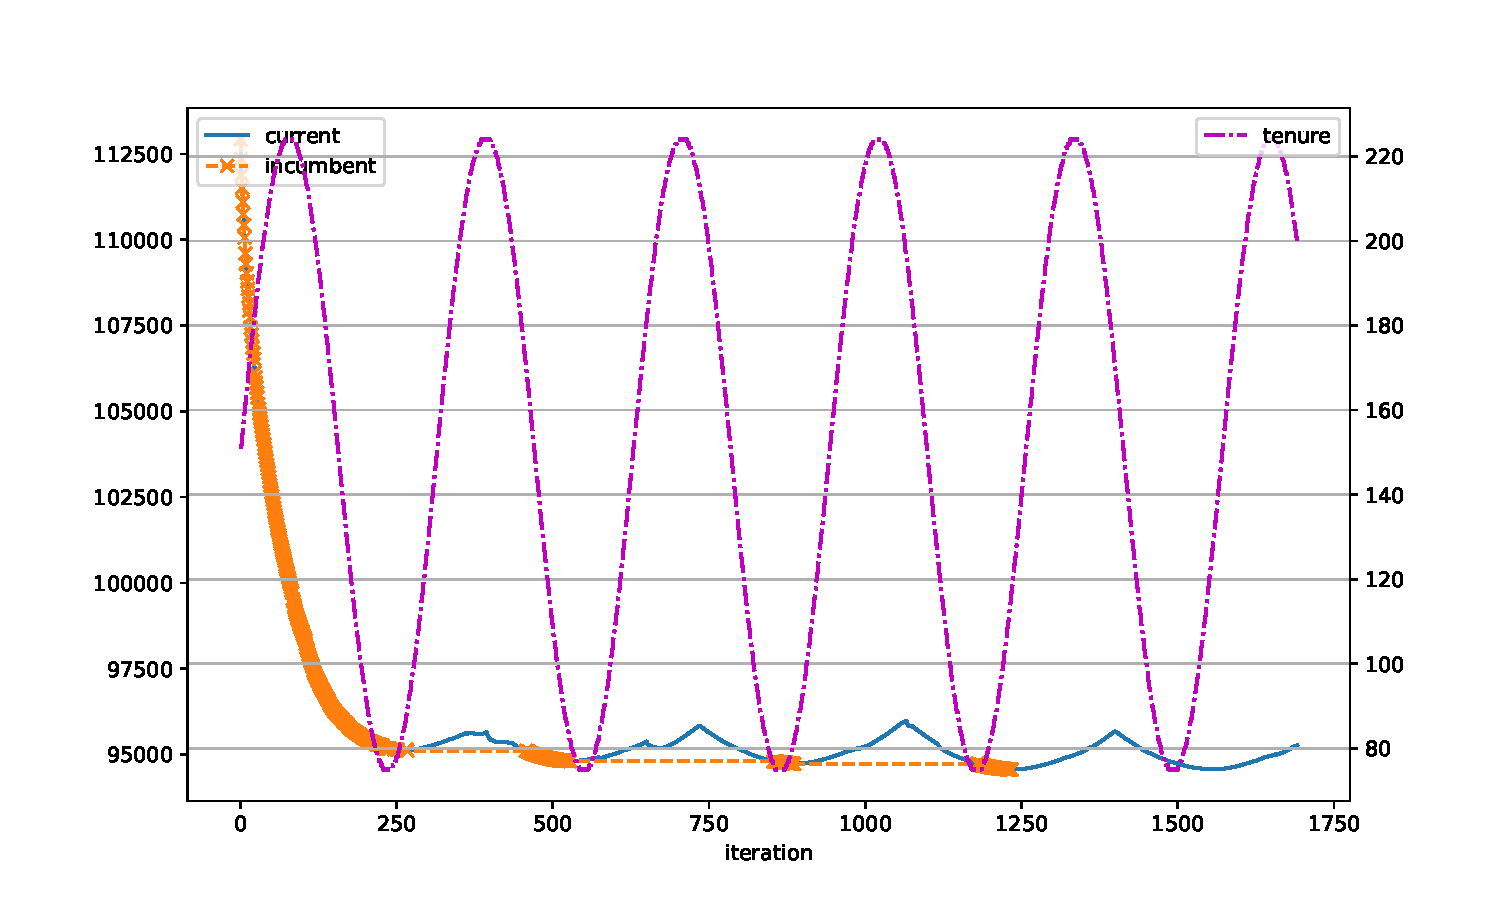
\includegraphics[width=400pt]{assets/sin_ten.pdf}
\end{figure}

\clearpage

\subsection{VNS (Variable Neighborhood Search)}
In \textit{Tabu Search} we have seen two different phases:
\begin{itemize}
        \item the \textit{Intensification Phase} to move towards a better solution
        \item the \textit{Diversification Phase} in which we try to escape from a local minimum using only
        non-tabu moves
\end{itemize}
With this approach, we may spend a considerable amount of time without achieving any improvement in
solution quality (Diversification Phase). One potential solution could involve restarting from a random
point each time we encounter a local minimum (Multistart). However, this approach would significantly
prolong the Intensification Phase. Moreover, when encountering a local minimum, it is probable
that the solution obtained is not entirely incorrect but requires adjustment in some aspect.
VNS is a metaheuristic that employs minimal permutations of the solution to evade local minima, as
opposed to restarting from a completely different starting point.
This technique was proposed by Mladenovi{\'c} and Hansen in 1997 \cite{mladenovic1997variable}.
With this approach, we transition from one solution to a better one using the 2-opt method until reaching
a local minimum. Subsequently, we perform a random number of permutations (called ``kicks'' in the following sections)
involving three nodes (3-opt) to navigate away from the minimum.
This approach also ensures that we never return to a previously visited
solution in the last 2-opt application, as it cannot be achieved through a sequence of permutations of
three nodes.
This is a simplified version of the algorithm; state-of-the-art techniques also allow for larger permutations
of nodes (e.g., 4-opt, 5-opt, etc.) instead of multiple 3-opt operations.
Algorithm~\ref{alg:vns} shows a very abstract description of the procedure

\begin{algorithm}[ht]
\caption{VNS}
\label{alg:vns}
\begin{algorithmic}
\Procedure{vns}{$solution$}
        \State\Call{greedy}{solution}
        \While{$!stop$}
                \State $move \gets \Call{findbest2optswap}{solution}$
                \State $delta \gets \Call{delta}{move}$
                \If{$delta \leq 0$}
                        \For{$\Call{random}{range}$}
                                \State $move \gets \Call{find3optswap}{solution}$
                                \State $solution \gets \Call{apply}{solution, move}$
                        \EndFor
                \Else
                        \State $solution \gets \Call{apply}{solution, move}$
                \EndIf
        \EndWhile
\EndProcedure
\end{algorithmic}
\end{algorithm}

The number of kicks is chosen randomly within a range, making the minimum and the maximum number
of kicks the only hyperparameters of this algorithm.
Tuning these hyperparameters can lead to better performance of the algorithm. Performing too many
kicks might result in restarting the intensification phase with a completely different solution,
prolonging the time spent during this phase, while performing
too few might not sufficiently change the solution, preventing us from visiting several different local minima.
The tuning of these hyperparameters will be discussed in Section \ref{sec:results}.

In Figure~\ref{fig:vns} it is possible to see an example of the solving procedure
using VNS. In this plot it is possible to see that, after the solver gets
stuck in a local minimum, it can escape it after a series of kicks.

\begin{figure}[ht]
        \caption{Example of VNS}
        \label{fig:vns}
        \centering
        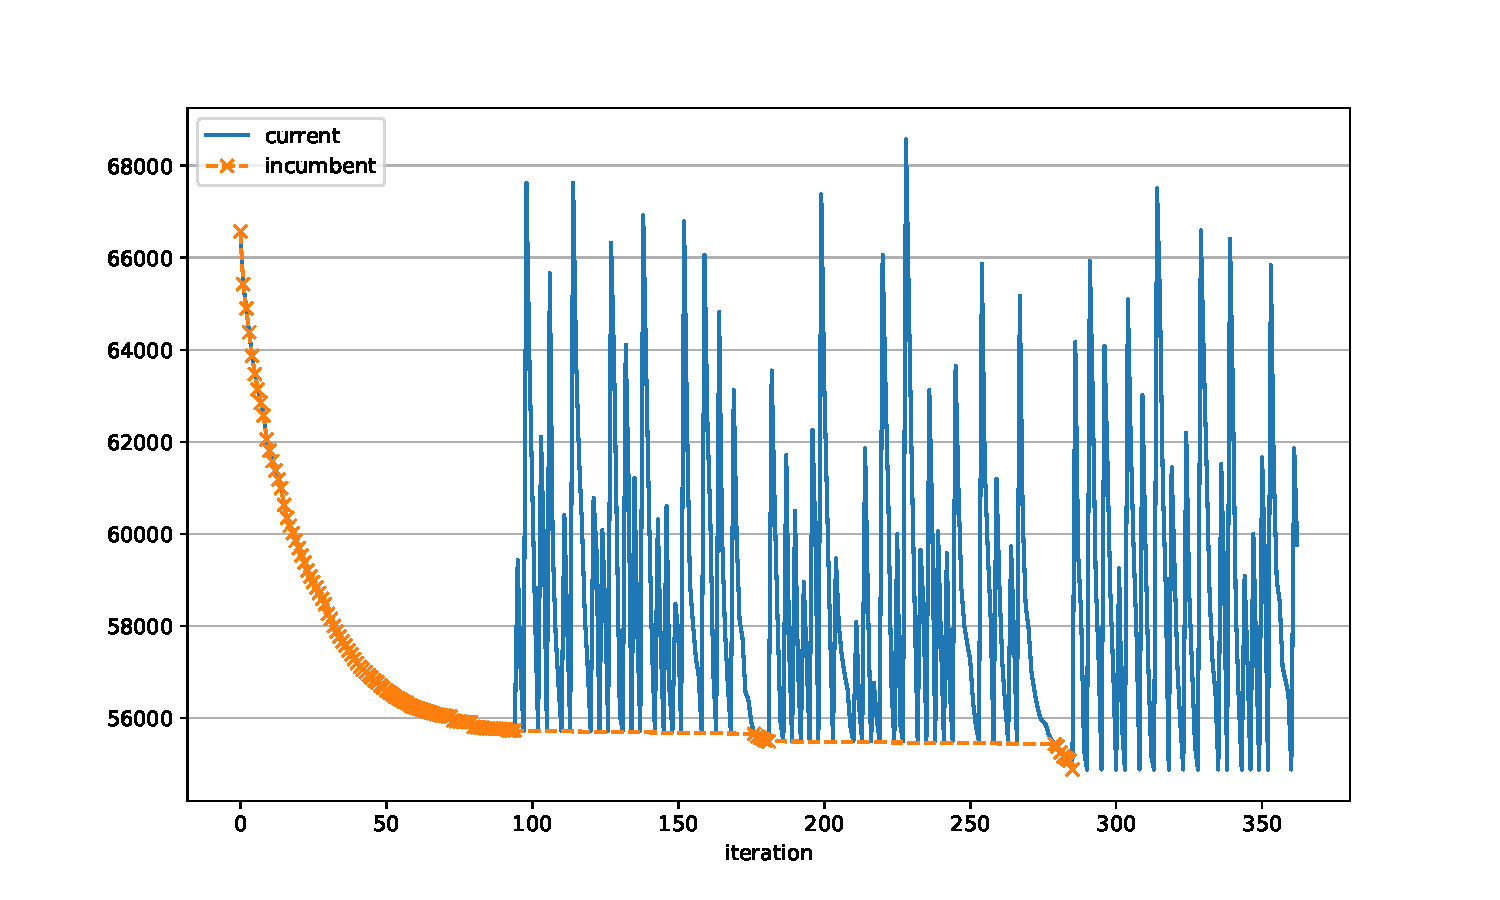
\includegraphics[width=400pt]{assets/vns.pdf}
\end{figure}

\clearpage

\section{Exact Methods}
Although, as we will see, a good heuristic can achieve very good results, it is also
important to consider approaches that lead to an optimal solution of the
TSP problem.

All of the techniques that we will cover are based on integer linear programming. It is
hence useful to provide an integer linear formulation for the problem.
Many formulations exist, but the one we will focus on is the one proposed by
Dantzig, Fulkerson and Johnson~\cite{dantzig1954solution}.

Initally we define an undirected complete graph $G=(V, E)$.
We will the use $c_e : E \rightarrow \mathbb{R}^+$ to indicate the cost of
an edge.
One of the ways to compute this cost function is to place all the points
on a 2d surface and compute their eucledian distance.

The variables of this model are
\begin{equation*}
        x_e =
        \left\{
                \begin{array}{l}
                1 \text{ the path uses edge $e$}\\
                0 \text{ otherwise }
        \end{array}
        \right.
\end{equation*}

The model, that makes use of the subtour elimination constraints, is the
following
\begin{equation}
  \begin{aligned}
\min & \sum_{e \in E} c_e x_e \\
\text{s.t.}
& \sum_{e \in \delta(h)} x_{e} = 2 \quad \forall h \in V \\
& \sum_{e \in E(S)} x_{e} \leq |S| - 1 \quad \forall S \subset V : |S| \geq 3 \\
& x_{e} \in \{0, 1\} \quad \forall e \in E.
\end{aligned}
\end{equation}
$\delta(h)$, where $h$ is a node, is defined as the set of edges that are
incident to $h$. $E(S)$, where $S$ is a set of nodes, is the est of all the
the edges with both extremities in $S$.

It is important to know that the number of SECs is exponential in the number of
the nodes. Hence, it is infeasible to generate all of them from the beginning
with the size of the instances we are interested in.

The techniques that will be shown in this section are different ways to generate
the subtour elimination constraints. We will use CPLEX to solve the MIP
problems.

CPLEX is a high-performance mathematical programming solver for linear
programming (LP), mixed-integer programming (MIP), and quadratic programming
(QP). When solving the TSP using CPLEX, we leverage its robust MIP solving
capabilities to handle the solution of the problem~\cite{cplex-docs}.
\subsection{Benders' loops}
\label{ssec:benders}
The first technique we will explore is the so-called ``Benders' loops'' technique.
The basic idea behind this approach is the iterated use of a MIP solver (like CPLEX)
as a black-box. More precisely, we will start by providing the solver with
a model lacking all the separation constraints. The solution of this model,
with all probability, is going to contain more than one loop. We will then
generate some constraints ``cutting'' the solution we have found.
The model, updated with the new constraints, is then passed to the solver
and solved again. This loop will be repeated until a solution composed by
only one component is found.
The process is described in Figure~\ref{fig:benders}.

\begin{figure}[ht]
        \caption{Solving using Benders' loops}
        \label{fig:benders}
        \centering
        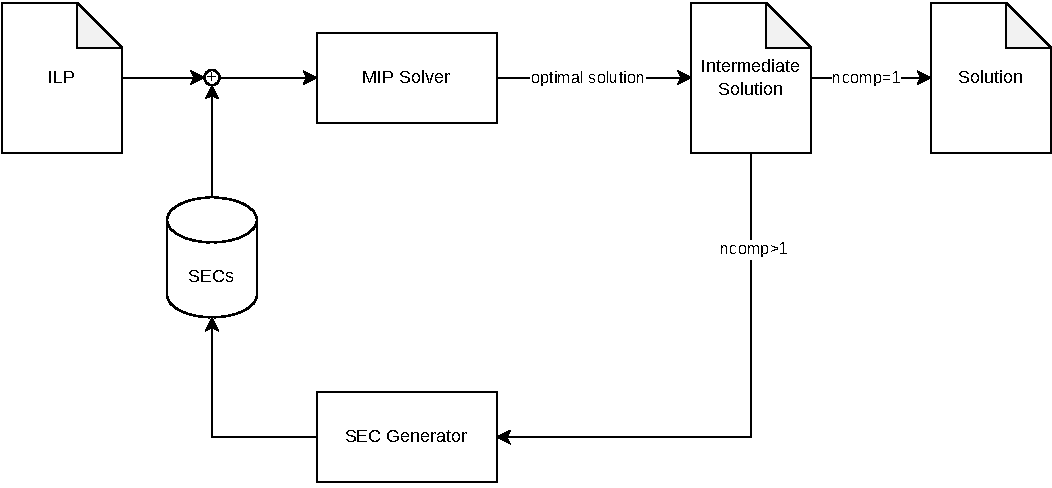
\includegraphics[width=340pt]{assets/bendersloops.drawio.pdf}
\end{figure}

It is very important to note that the ``optimal solution'' output of the
MIP solver is not the optimal solution of the TSP problem (exception made
for the last iteration of the loop). That solution is optimal only for the
current set of subtour elimination constraints.

As we will see in Section~\ref{sec:results}, although this method allows us to
solve some instances it has a major flow. By using the MIP solver as a black
box, we have to restart all the process every time a new solution (that
contains subtours) is found. This creates one big problem: the branch-and-bound
tree will be discarded and the search for the optimal solution will start again.
Even though throwing away the search tree can be sometimes beneficial~\cite{achterberg2009scip}\cite{achterberg2007constraint},
it needs to be done following some precise criteria and at the correct time.

\subsubsection{Patching}
\label{sssec:patching}
At the end of the Bender's loop we are guaranteed to obtain a solution to the TSP problem.
However, if we finish the procedure earlier because of the time limit, we'll return a solution containing more than
one loop. To solve this problem we implemented the so-called ``Patching Heuristic''.
The idea behind this algorithm is to find a way to merge together all the components returned by the MIP solver
so that, at each iteration of the Bender's loop, we have a solution composed of only one component.
In this way, if we exit the Bender's loop because of the time limit, we'll always be able to return a
correct solution to the problem.
Figure \ref{fig:patching} shows an example of patching.

\begin{figure}[H]
        \caption{Example of patching}
        \label{fig:patching}
        \centering
        \begin{subfigure}{.5\textwidth}
                \centering
                \def\svgwidth{.7\linewidth}
                \import{assets}{pre_patching.pdf_tex}
                \caption{MIP solver solution}
        \end{subfigure}%
        \begin{subfigure}{.5\textwidth}
                \centering
                \def\svgwidth{.7\linewidth}
                \import{assets}{post_patching.pdf_tex}
                \caption{Patched solution}
        \end{subfigure}
\end{figure}

The Patching Heuristic aims to find the optimal way to merge two different components. As shown
in Figure \ref{fig:patching}, the patched solution is the one that minimizes the cost of the
resulting single component.

The solution to the TSP is an \textit{undirected graph} because
we are considering instances of the \textit{symmetric TSP} problem.
However, in our implementation, such solution is stored as a permutation of the nodes and
so, implicitly, we have a \textit{directed graph} as solution to the problem.
If we have two loops running in opposite directions, it could be that the
patched solution is not the optimal one (because of an intersection of the newly added edges).
To address this issue, after each patching step we apply a 2-opt optimization to refine the solution.

An abstract description of the techinque is presented in Algorithm \ref{alg:patching}.

\begin{algorithm}[ht]
\caption{Bender's loop + Patching Heuristic}
\label{alg:patching}
\hspace*{0.5em} \textbf{Output}: $solution$
\begin{algorithmic}
\Procedure{benders+patching}{$model$}
        \While{$!stop$}
                \State $solution \gets \Call{mipsolver}{model}$
                \If{$\Call{components}{solution} == 1$}
                        \State $break$
                \EndIf
                \State $model \gets model \cup SEC$
                \State $solution \gets \Call{patchcomponents}{solution}$
        \EndWhile
\EndProcedure
\end{algorithmic}
\end{algorithm}

\subsection{Opening CPLEX}
The title of this section refers to the fact that, to improve what we did in the
previous section, we use and approach where we need to interact with CPLEX and
control its exectuion.

The technique that will be presented in this section solves the problem
described in Section~\ref{ssec:benders} by generating the constraints when
the MIP solver finds a new canditate solution. In order to achieve this,
CPLEX provides us a C interface that we can use to control the execution
of the branch-and-cut.

The process will go as follows: first, we will provide the solver with the
ILP model, without the cuts. Whenever the solver finds a candidate solution,
the execution will be passed to a function that we have defined.

We will need a way to generate valid cuts
whenever the MIP solver has a new canditate solution. To do this we ``install''
a callback. CPLEX allows us to pass a function to it, that will be called when
a specific condition is met. In our case we will use one\footnote{CPX\_CALLBACKCONTEXT\_CANDIDATE} that is called when CPLEX
has found a new candidate for an integer-feasible solution.

Inside this function we will count the number of components. If the number of
components is greater than one, we will generate the corresponding subtour
elimination constraints and reject the solution.

It is possible to see a diagram of such process in Figure~\ref{fig:callback}.

\begin{figure}[ht]
        \caption{Solving using candidate callback}
        \label{fig:callback}
        \centering
        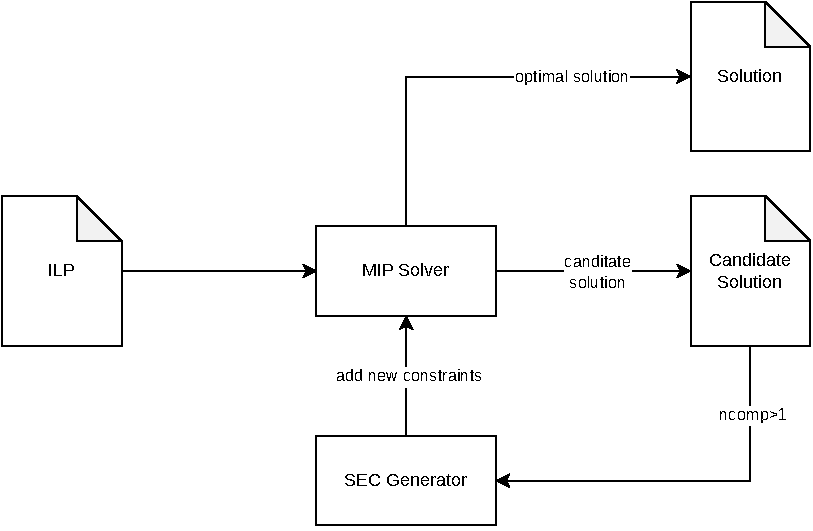
\includegraphics[width=340pt]{assets/callback.drawio.pdf}
\end{figure}

\clearpage

Even though, as we will see in Section~\ref{sec:results}, the method mentioned
above allows us to obtain satisfying results, there exist ways to improve it
even more. Three of these methods will be covered in this report.

\subsubsection{Warm start}

The first method involves providing the MIP solver with a starting solution, known as a
``warm start''.
CPLEX will save this solution in its ``solution pool'' and will be able to use
it if it can be useful.
The MIP solver will process the provided solution before starting the branch-and-cut algorithm,
giving it an incumbent solution, that can help eliminating portions
of the search space, potentially resulting in a smaller branch-and-cut tree.

\subsubsection{Solution posting}

The second method is the ``heuristic solution posting'', where heuristic solutions are provided to the solver during the optimization process.

The procedure we developed works as follows: everytime the callback function
is executed, as we have previously seen, CPLEX will have found a solution
formed by many subtours. After generating the SECs, we can leverage the
method we have described in Section~\ref{sssec:patching} to ``glue'' the subcycles
together and obtain a feasible solution. We will see in
Section~\ref{sec:results} that \textit{posting} this solution to CPLEX can
be beneficial to the process.


\subsubsection{Fractional cuts}
The third and last method we tried was the generation of violeted cuts from the relaxed
solutions CPLEX runs into.
In order to do so, we use a callback\footnote{CPX\_CALLBACKCONTEXT\_RELAXATION} that is
invoked whenever CPLEX has found a relaxed solution.
This solution is usually not integer and, most of the times, comes from the solution
of a node LP-relaxation.

It is possible to show that \textit{the separation problem for finding a violated subtour elimination
constraint can be reduced to a maximum flow problem}.
To accomplish this we used a routine from the Concorde~\cite{applegate1998solution} software to solve such maximum flow problem,
corresponding to the LP relaxation of our TSP problem.

This procedure involves the function \verb|CCconnect_components|,
which identifies connected components in the graph, and \verb|CCviolated_cuts|, which generates violated cuts.

By using these functions we can add SECs derived from the fractional solution of the an integer relaxation
of the problem, rather than from the integer solution.

Generating cuts from these solutions can help the solver to narrow down the size of the search space, eliminating
useless branches early. Hence the algorithm can converge to the optimal solution more efficiently.

Since this procedure is time consuming, we cannot afford to execute it on every
node of the branch-and-cut tree. Our approach was to apply it only on the
solutions generated by a subset of the nodes. We arbitrarily decided to perform
it on a tenth of the nodes, using the modulo operator to decide which ones. In
our implementation, the relaxed solutions coming from a node with index divisible by $10$,
will go through this procedure.

\newpage

\section{Matheuristics}
In this section we will explore another useful set of techniques that we will call
\textit{matheuristics}.
The core idea behind these techniques is to use heuristics in conjunction with the
mathematical models that one would normally use to solve the problem optimally.
One of the advantages of such approaches is that they can be applied to different problems,
with little to none needed adaptations.

What is important to note here is that matheuristics isn't a new class of techniques
for solving optimization problems but it is instead a nomenclature that was given
to the concept of using mathematical tools to design heuristics~\cite{boschetti2022matheuristics}.

The term was coined to give a name to the first edition of a workshop in Bertinoro, Italy
in 2006.

In this report we will focus on two matheuristic techniques.
The first one that will be explored is Diving, while the second one is Local Branching.

As we will see in Section~\ref{sec:results}, these techniques will be used to solve
heuristically instances bigger than what we will be able to solve optimally using approaches
based on the branch-and-cut.

\subsection{Diving}
The first technique that we are going to explore is \textit{Diving}.

\textit{Diving} is a refinement algorithm, meaning that it is a way to improve a feasible
sub-optimal solution.

The idea goes as follows: we start from a solution (that can be obtained with an heuristic or in
the worst case generated randomly) and we fix part of the selected edges. The fixing of the
edges will be done by adding constraints to the model, allowing us to use the MIP solver
as a black box.

We can fix all the edges
\begin{equation*}
  x_{e}=1 \quad \forall e \in \tilde{E}
\end{equation*}
where
\begin{equation*}
  \tilde{E} \subset E^{H} \coloneq \left\{ e \in E : x_{e}^{H} = 1 \right\}
\end{equation*}
meaning that the edges we fix are a subset of the edges that are part of the heuristic solution.

It is important to note that only the edges with a value of 1 are fixed. We
decide to focus on ``positive'' decisions to avoid overly constraining the
subproblem, thereby maintaining a more flexible and effective search space that
enhances the chances of finding optimal or near-optimal solutions \cite{maniezzo2021diving}.

What is left now is deciding how many and which edges to fix. The approach that will be explored
in this report is choosing a number of edges (which will become an hyperparameter of our system)
and select the edges to fix randomly.

Figure \ref{fig:diving} shows a description of the process.

\begin{figure}[H]
        \caption{Diving}
        \label{fig:diving}
        \centering
        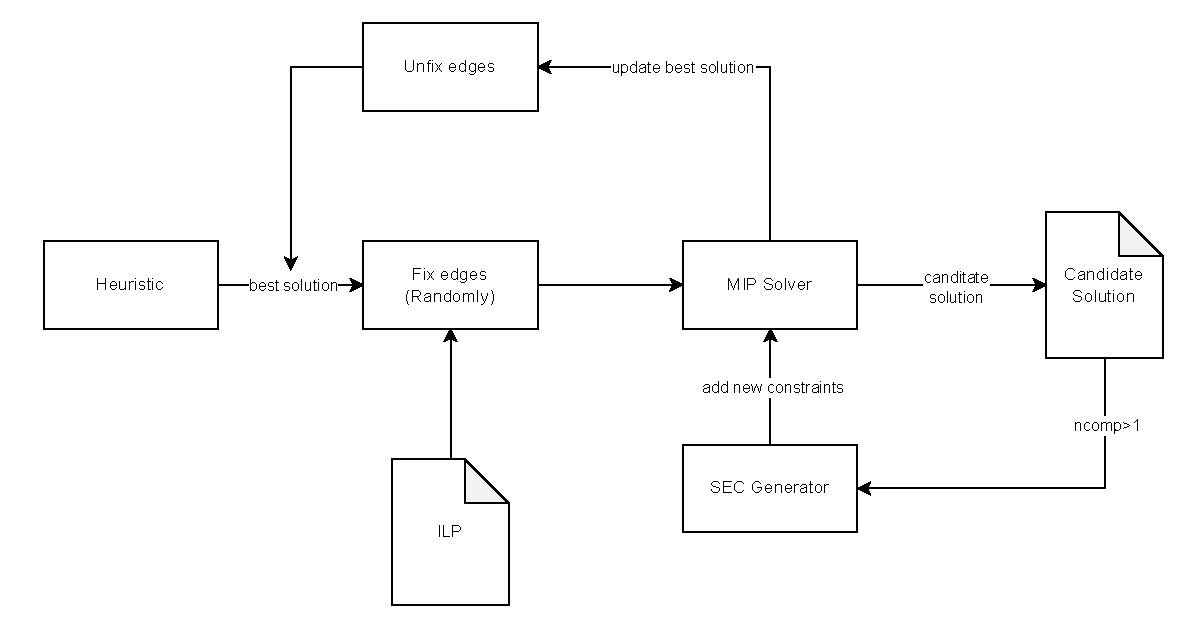
\includegraphics[width=340pt]{assets/diving.drawio.pdf}
\end{figure}

\subsection{Local Branching}
The second approach this report will focus on is \textit{Local Branching}.

\textit{Local Branching} was initially introduced in a paper by Fischetti and Lodi~\cite{fischetti2003local} and was then applied by many other researchers over the following
years.

The idea behind this technique is to decide the number of edges to fix, like we did for Diving,
but then leaving the choice of \textit{what edges} to the MIP solver.

This is possible thanks to the Local Branching constraints, which, in their simplified
asymmetric version are constructed like this

\begin{equation*}
        \sum_{e : x_{e}^{H}=1} x_{e} \geq n - k
\end{equation*}

This forces at least $n-k$ edges of the heuristic solution we apply this method on to be
set to $1$ in the solution of the model this constraint is part of.

We say that this is an \textit{asymmetric} version because the ``original'' Local Branching
constraint would consider also the variables set to $0$ becoming $1$.
In the TSP problem it would make no sense to add such constraints since every feasible
solution has the same number of variables set to $1$.

The \textit{simplified} comes instead from the fact that we know a priori the number of
variables set to $1$ in a solution. This allows us to put $n$ directly into the right-hand-side
of the constraint and avoid building a more complicated cut where we consider the difference
of variables set to $1$ between the input heuristic solution and the solution of the model.

In its original version the Local Branching constraint introduced by Fischetti, that
could be written as
\begin{equation*}
\sum_{i \in I: \hat{x}_i = 0} x_i + \sum_{i \in I: \hat{x}_i = 1} (1 - x_i) \leq k \text{,}
\end{equation*}
limits the Hamming distance between the heuristic and the solution we will find to
a value $k$.

This can be seen as a technique to use the MIP solver as a black box to find
the best $k$-opt moves in a feasible solution.

This leaves us with one hyperparameter to tune: the value of $k$ for each iteration.
Our approach in this report will be to decide an initial value of $k$ that we will call
$k_{0}$. The first iteration of the local branching will use $k_{1} = k_{0}$.
We will keep running the solver with the same value of $k$ until no improved
solution can be found. At this point, say iteration $t$, we increment $k$ by a delta:
$k_{t+1} = k_{t} + \Delta k$. This process will continue until we reach the timelimit.

\newpage

\section{Results}
\label{sec:results}
This section is structured as follows: first we will try to optimize the hyperparameters
of the approaches that have some. Then, we will compare the methods in their best configuration,
searching for the best one.

Naturally, the main difference we have among the approaches that we present is if we are computing
an optimal solution or if we are applying an heuristic. In the former case, the metric we are going
to compare our systems on is the time it took them to arrive to the optimal solution.
For the latter we instead fix a time limit (the maximum time we allow our system to run for) and
we seek the system that found the best solution (in our case the smallest one, since the TSP
is a minimization problem).

It is important to know that we set a timelimit also for the exact method. This
needs to be done for practical reasons while running the experiment.

Before going through the experiments that were performed, it can be useful to discuss some
parameters that will be used in this section.
The instances will be generated randomly and we will refer to them using the seed we
initialize our number generator with.
The size of the instances will be
\begin{itemize}
        \item $300$ for the optimal methods
        \item $1000$ for matheuristics
        \item $1500$ for heuristics
\end{itemize}

For what concernes the value of the time limit, we will use $120$ seconds for all the
experiments.

To make comparisons a little bit more statistically valid, all the systems will be run on
$20$ different instances of the same size. We will then take the results for each instance
and plot the Performance Profile. All our considerations will be based on these plots.

It is also important to discuss how the distance between the points in the 2d
grid was computed: in our experiments we use the ATT formula from the TSPLIB~\cite{reinelt1991tsplib}.

\subsection{Experimental Setup}
All the experiments were run on the same machine equipped with an Intel Core i7 6700k
and 16GB of RAM. The MIP solver used was IBM ILOG CPLEX 22.1.0~\cite{cplex-docs}.

\subsection{Performance profile}
Performance profiles are graphical representations used to compare the performance of different algorithms
across multiple problem instances.
In these plots, each algorithm is represented by a line, where a point (x, y) indicates that: \textit{the algorithm achieves
a solution within a factor of x of the best observed performance for y percentage of the problem set}.
Therefore, using these plots allows for identifying which algorithm is consistently better across a range
of problem instances. We will use them widely in the next sections for hyperparameter tuning and
to determine the best method among different algorithms.
To determinte the best algorithm we will use two different metrics based on the type of algorithms
under study: for heuristics and matheuristics, we use the cost of the solution found as the metric, while
for the exact methods, we are going to use the time spent to find the optimal solution.

\subsection{Hyperparameters tuning}
Before comparing the methods with each other, it is useful to discuss some
of the hyperparameters these approaches require.

\subsubsection{Greedy}
With regard to the greedy approach, the hyperparameter we should tune is
deciding whether or not to use the 2-opt procedure. We can see the plot
in Figure~\ref{fig:ht_greedy}. From this performance profile we can conclude
that using the 2-opt procedure is beneficial to the cost of the best
solution we can find.

\begin{figure}[ht]
        \caption{Performance profile of the greedy approaches}
        \label{fig:ht_greedy}
        \centering
        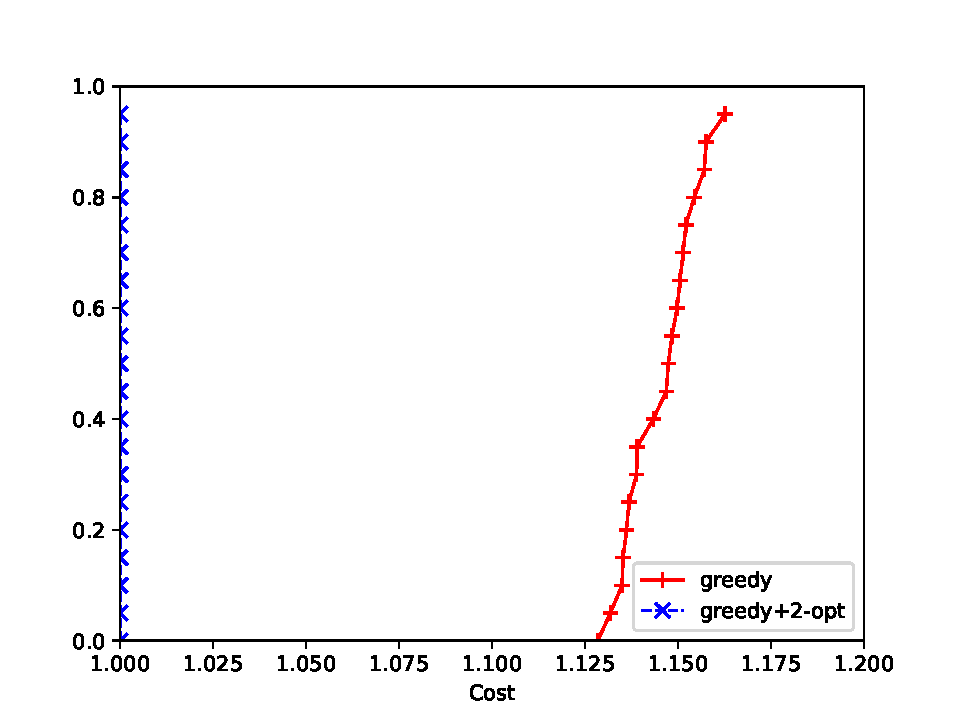
\includegraphics[width=340pt]{assets/ht_greedy.pdf}
\end{figure}

Specifically, integrating the 2-opt algorithm resulted in a notable improvement of 12\% in solution cost.

\clearpage

\subsubsection{Tabu search}
On the subject of Tabu Search, there are a few hyperparameters we need to tune:
we need to discuss what the size of the tenure will be. In our
experiments we will explore two different approaches: the first one will use
a fixed value of the tenure for the whole experiment. The second approach we
will cover is to use a sinusoidal value for the tenure.

In the first case there will be only the value of the fixed tenure to tune.
The size of the tenure $T$ is computed as follows.

\begin{equation*}
        T = \max \left\{
                \frac{n}{\alpha_0} ,
                T_{min}
        \right\}
\end{equation*}
where $n$ is the number of nodes, $T_{min}$ is the minimum value for the tenure
and $\alpha_0$ is the parameter we want to tune. The value of $T_{min}$ is arbitrarily
set to $10$.

The performance profile for this parameter is presented in Figure~\ref{fig:ht_fixten}.

\begin{figure}[ht]
        \caption{Performance profile of the fixed Tabu Search on the parameter $\alpha_0$}
        \label{fig:ht_fixten}
        \centering
        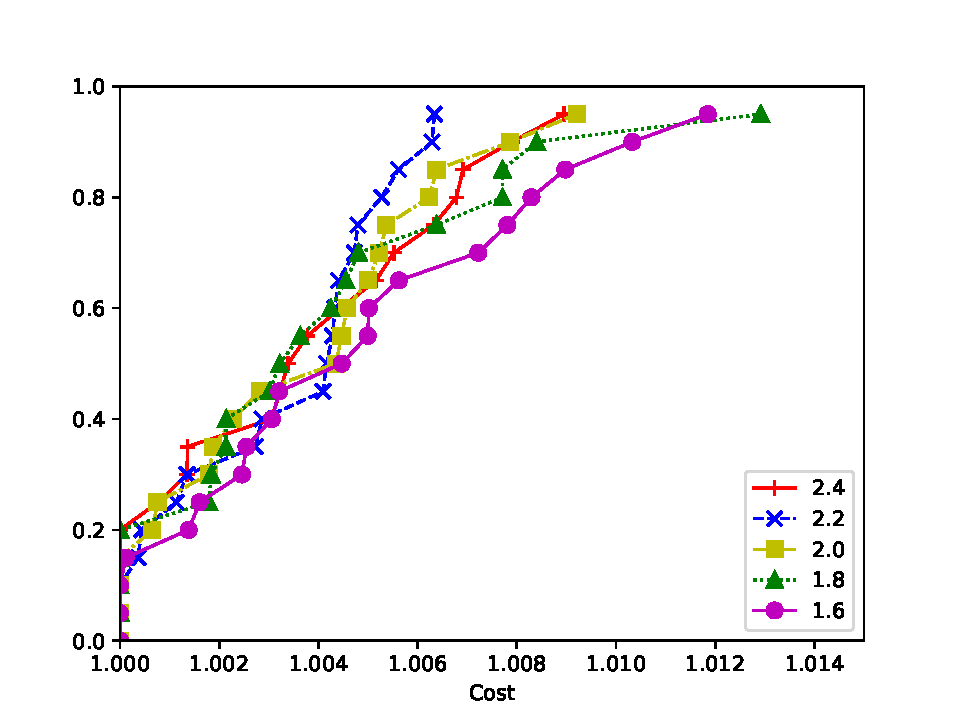
\includegraphics[width=340pt]{assets/ht_fixten.pdf}
\end{figure}

Although all parameters yield very similar performances, the Tabu Search with $\alpha_0 = 2.2$
appears slightly superior to the others. Therefore, we will adopt this parameter for the subsequent experiments.

\clearpage

With regard to the second approach, we have more than one parameter. First of
all we will need to decide the parameters for the sinusoidal function. In our
case the value of the tenure $T$ will be computed on the base of the current
iteration $i$. We will also include the number of nodes $n$ and two parameters
that we will use to scale the sinusoidal function, $\alpha_1$ and $\alpha_2$.
Another parameter that will be used is a minimum value for the tenure,
indicated with $T_{min}$. In our experiment we set this value to $10$.

First of all we compute the value of the scale $s$:

\begin{equation*}
        s = \frac{n}{\alpha_1}
\end{equation*}

Then we can compute the value of the tenure:

\begin{equation*}
        T = \max \left\{
                \sin \left( \frac{i}{\alpha_2} \right) \cdot s + 2 s ,
                T_{min}
        \right\}
\end{equation*}

The performance profile for this parameter is presented in Figure~\ref{fig:ht_fixten}.

\begin{figure*}[ht]
        \caption{Performance profile of the sinusoidal Tabu Search on the parameters $\left(\alpha_1; \alpha_2\right)$}
        \label{fig:ht_sinten}
        \centering
        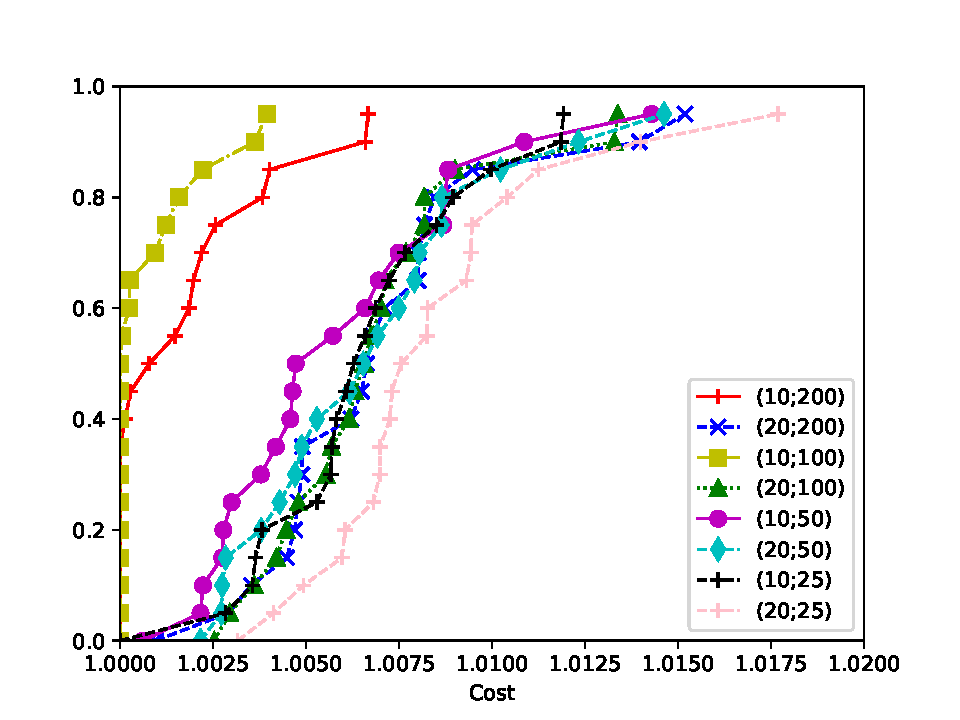
\includegraphics[width=340pt]{assets/ht_sinten.pdf}
\end{figure*}

Tabu Search with sinusoidal tenure parameters (10;100) and (10;200) exhibit significantly better performance compared to the others.
The set of parameters (10;100) appears slightly superior to the other one. Therefore, we'll use these parameter for the
subsequent results.

\clearpage

\subsubsection{VNS}
The parameter we have to tune for the VNS is the number of ``kicks'' we apply
after reaching a local minimum. Since in our implementation we generate a
random number of kicks to be applied, we have two parameters to tune: the
minimum the maximum number of kicks.
The performance profile for this experiment is shown in Figure~\ref{fig:ht_vns}.

\begin{figure*}[ht]
        \caption{Performance profile of the VNS on the parameters $\left(min; max\right)$}
        \label{fig:ht_vns}
        \centering
        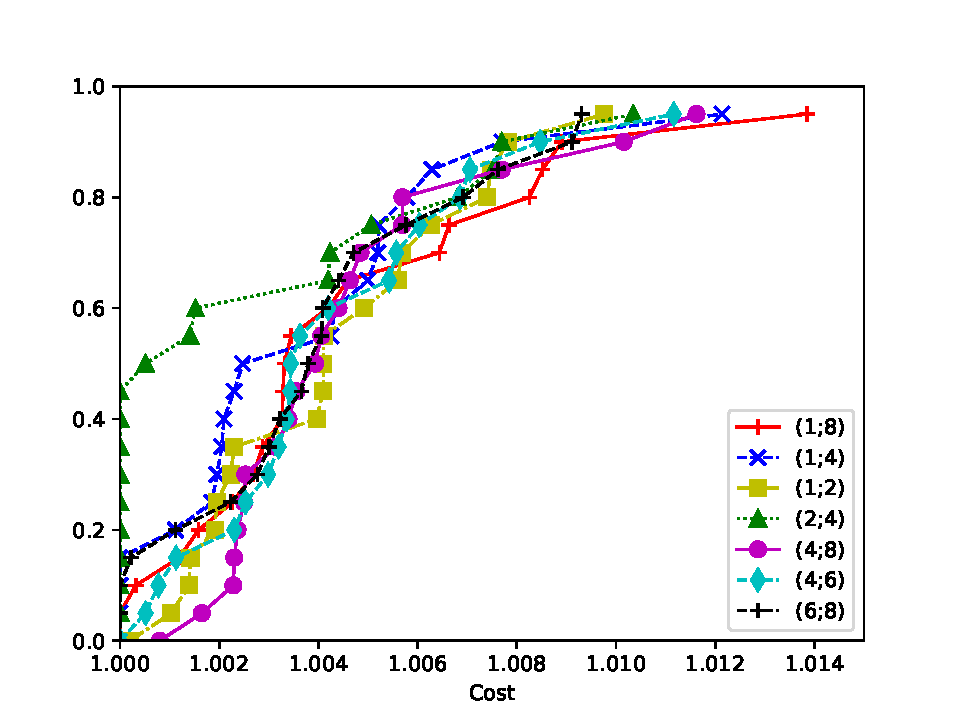
\includegraphics[width=340pt]{assets/ht_vns.pdf}
\end{figure*}

In this scenario, the performance of all parameters is quiete comparable. For the following results, we decided to use
VNS with parameter (2;4) as it demonstrates better performance across most cases.

\clearpage
\subsubsection{Fast-heuristic}
Since for the next experiments we will need an heuristic to run for a tenth of
the total available timelimit, we are going to discuss what is the best
procedure we can use to find the first heuristic solution. The total available
runtime is $120$ seconds, so we will compare the heuristics we discussed so far
on a $12$ seconds timelimit.

Since this heuristics will be used as an initial phase for matheuristic,
the experiments were run with $1000$ nodes.

To avoid comparing all the heuristics again, we picked one or two (in the case
a clear winner is not present) from every approach.

The label in the legend should be interpreted as the name of the method (as
covered in the previous sections) followed by the parameters, if present.
\textit{tabu\_f} refers to the Tabu Search using a fixed tenure while
\textit{tabu\_s} refers to the sinusoidal tenure version.

\begin{figure*}[ht]
        \caption{Performance profile of the heuristics with $12$ seconds}
        \label{fig:ht_best12}
        \centering
        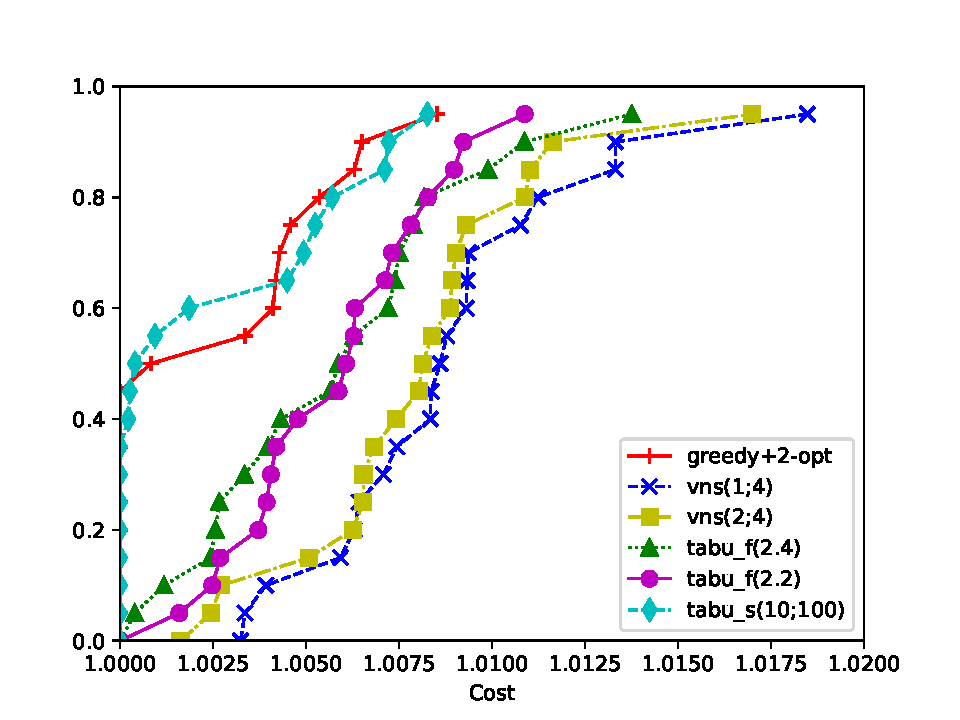
\includegraphics[width=340pt]{assets/ht_best12.pdf}
\end{figure*}

From the plot we can see that the two best performing approaches are the greedy
with 2-opt and Tabu Search with a sinusoidal tenure with parameters
$\left(\alpha_1; \alpha_2\right) = \left(10;100\right)$.
By interpreting this plot, we decided to use greedy in conjunction with 2-opt
as the initial heuristic for the next experiments.

\clearpage
\subsubsection{Diving}
With regard to the diving algorithm, we need to tune the percentage of edges to fix
in the starting solution provided by the greedy + 2-opt algorithm
to enable the MIP solver to handle the otherwise too large problem.
The results are shown in the performance profile in Figure \ref{fig:ht_diving}

\begin{figure*}[ht]
        \caption{Performance profile of Diving}
        \label{fig:ht_diving}
        \centering
        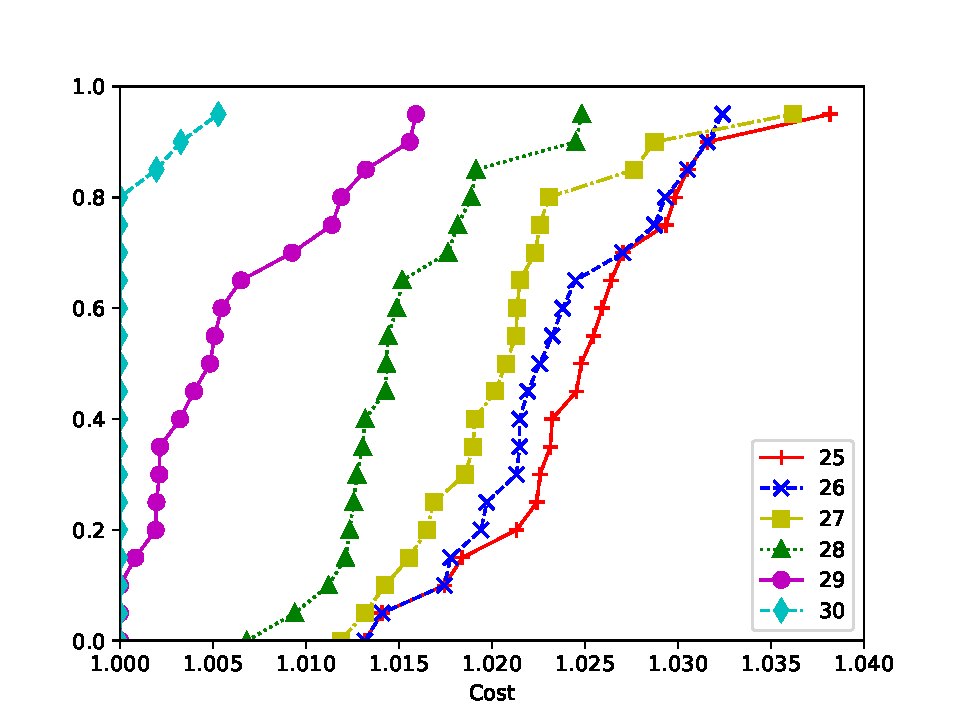
\includegraphics[width=340pt]{assets/ht_diving.pdf}
\end{figure*}

Fixing too many edges of the provided solution (80\%, 90\%) leads to the worst performance. This may be because
the MIP solver struggles to find a good solution due to the limited degrees of
freedom we allow it. Instead, fixing the 40\% of the edges belonging to the solution, and hence giving
CPLEX more degrees of freedom, leads to the best performance.

\clearpage
\subsubsection{Local branching}
As we mentioned in Section \ref{fig:ht_localb}, the local branching algorithm depends on two hyperparameters:
the initial number $k_0$ of edges to be fixed and the $\Delta k$ used to increment the generic
$k_t$ when an improved solution is found.
Figure \ref{fig:ht_localb} shows the performance profile for tuning $k_0$.
For simplicity, $\Delta k$ is arbitrarily set to 5.

\begin{figure*}[ht]
        \caption{Performance profile of Local Branching}
        \label{fig:ht_localb}
        \centering
        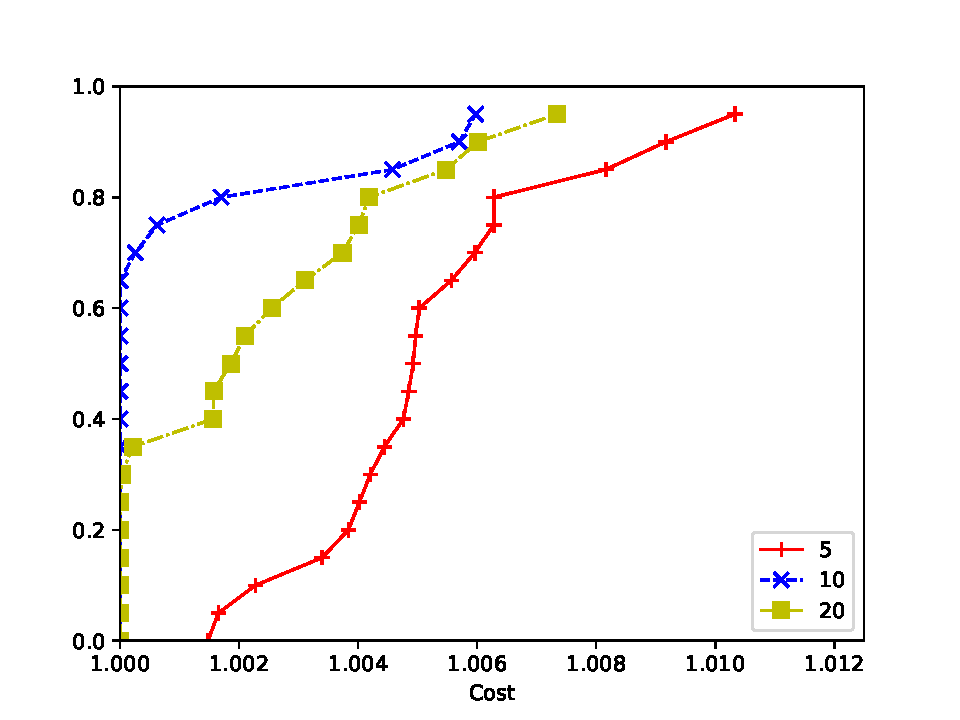
\includegraphics[width=340pt]{assets/ht_localb.pdf}
\end{figure*}

The best performance is obtained by setting $k_0 = 10$, so we will use this parameter
to compare it with the other matheuristics.

\clearpage
\newpage
\subsection{Best heuristic}

In this section we will show a comparison between the best hyperparameter
configuration for the presented heuristic techniques.
Figure \ref{fig:res_bestheu} depicts the performance profile among
all the heuristic algorithms discussed previously.

\begin{figure*}[ht]
        \caption{Performance profile among the different approaches}
        \label{fig:res_bestheu}
        \centering
        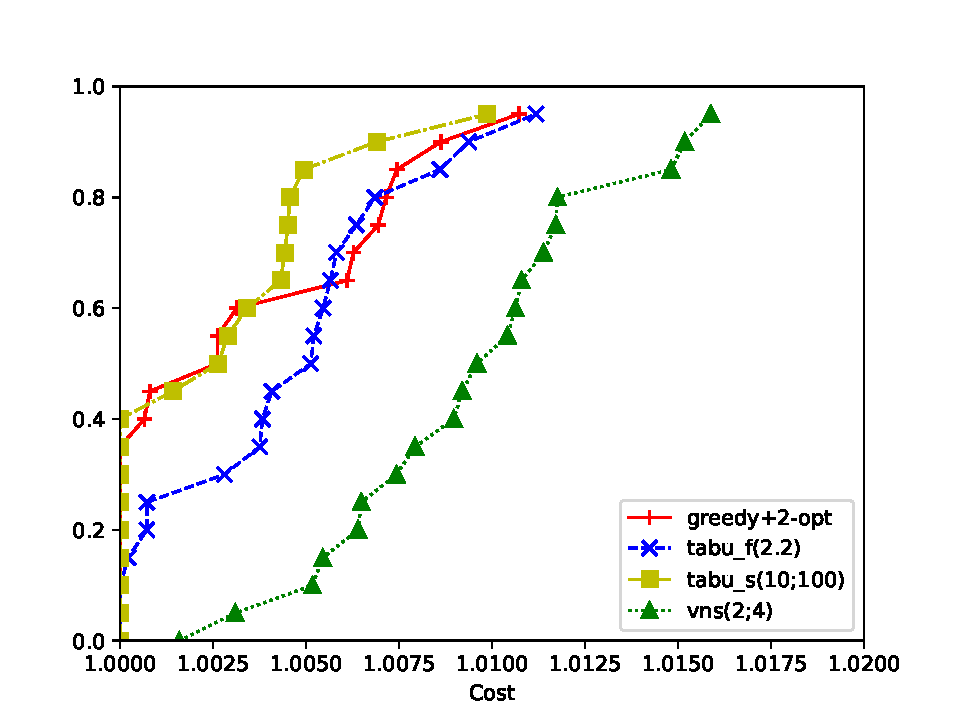
\includegraphics[width=340pt]{assets/res_bestheu.pdf}
\end{figure*}

Greedy + 2-opt and Tabu Search with sinusoidal tenure exhibit very similar performance
across most instances, while VNS and Tabu Search with fixed tenure are less effective.
In the end, the Tabu Search with sinusoidal tenure stands out as the best heuristic
because it consistently performs above the other curves across nearly all
instances.

\clearpage
\newpage

\subsection{Best exact method}
In this section we will show a comparison between all the exact methods
we discussed previously.
The following clarifies the meaning of the curve labels shown in Figure \ref{fig:ht_bec}:
\begin{itemize}
\item base: branch-and-cut
\item warm: branch-and-cut with warm start
\item frac: branch-and-cut with fractional cuts
\item post: branch-and-cut with heuristic solution posting during the execution
\item bl: Benders' loop
\end{itemize}

\begin{figure*}[ht]
        \caption{Performance profile of the various branch-and-cut techniques}
        \label{fig:ht_bec}
        \centering
        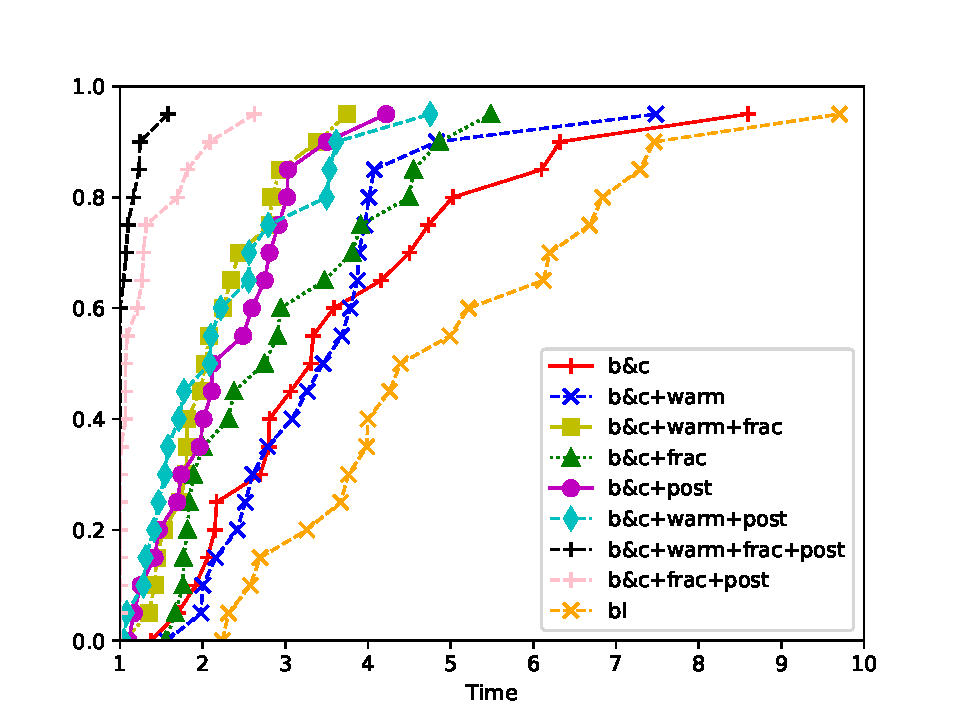
\includegraphics[width=340pt]{assets/ht_bec.pdf}
\end{figure*}

Every branch-and-cut variation have better performance compared to the Benders'
loop technique. While warm start does not significally improve the performance of the
branch-and-cut, fractional cuts and heristic solution posting variations show better results.
The combination of all these techniques proves to be the most effective.

\clearpage
\newpage

\subsection{Best matheuristic}
In this section we'll show a comparison between all the matheuristic algorithms
we presented.
Figure \ref{fig:math_vs_tabu} shows the performance profile of these techniques.
For reference, it shows also what the best heuristic (Tabu Search with sinusoidal tenure)
would have performed compared with the matheuristic algorithms.

\begin{figure*}[ht]
        \caption{Performance profile of the various matheuristic techniques, along with the best heuristic}
        \label{fig:math_vs_tabu}
        \centering
        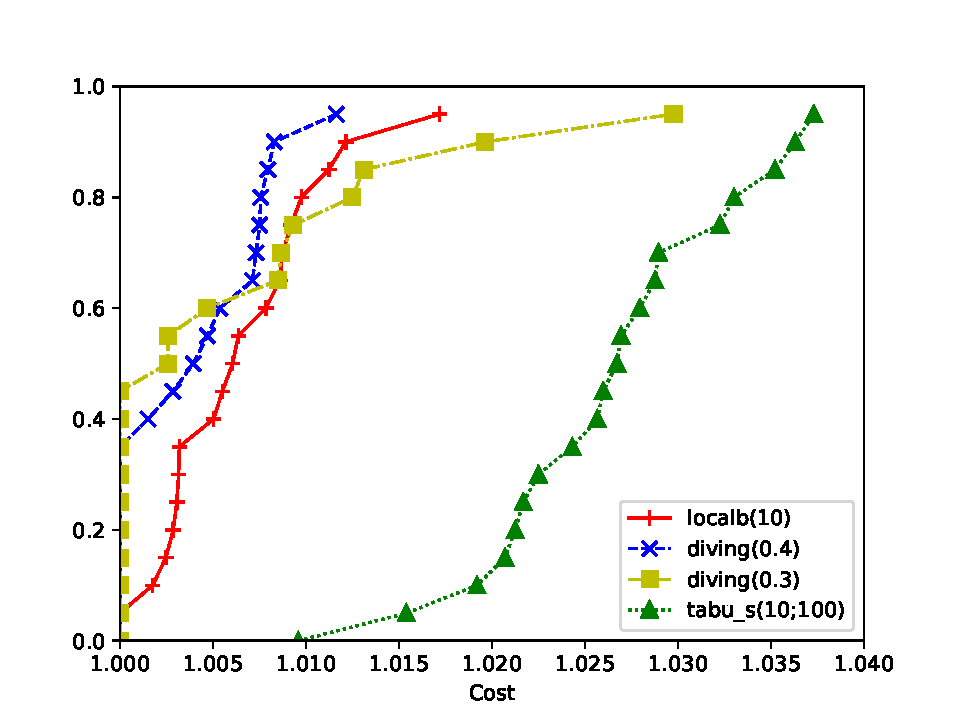
\includegraphics[width=340pt]{assets/math_vs_tabu.pdf}
\end{figure*}

The matheuristic algorithms outperform the Tabu Search.
Among them, the diving methods demonstrate superior performance compared to the local branching method.

\clearpage
\newpage

\bibliographystyle{plain}
\bibliography{thesis}

\end{document}
